\section{ARM}
L' architettura ARM sta per ACORN Risc Machine ed è prodotta dalla ex ACORN ora ARM.
Fu inizialmente prodotta per la realizzazione dell' ACORN Archimedes che fu un fiasco perché fu venduto con un sistema operativo parziale, successivamente fu utilizzato sulla prima versione dell' ACORN BBC, richiesto dalla BBC per poter fare un corso sui computer utilizzando hardware sotto i 1000£.
Successivamente un' altra azienda ha comperato il progetto di ARM in cambio di 0,20£ per ogni pezzo venduto.

Ci sono varie versioni di ARM con alcune specifiche per uC:
\begin{itemize}
    \item Cortex M: sono microcontrollori
    \item Cortex R: serie speciale ad alta affidabilità usati in contesti industriali
    \item Cortex A: usati per computer, tablet e cellulari
\end{itemize}

\subsection{Caratteristiche}
Sono processori a 32 bit, ma ora ci sono anche le versioni a 64 bit (aarch64), quindi hano 32 linee di indirizzo e permettono di usare al massimo 4GB di RAM.
Hanno una architettura di Von Neumann quindi c'è solo uno spazio di memoria e si può indirizzare direttamente il byte.

Permette esclusivamente accessi allineati:
\begin{itemize}
    \item byte per un indirizzo qualsiasi
    \item word se allineato a 2
    \item quad word se allineato a 4
\end{itemize}

Le istruzioni sono tutte a 32 bit ed abbiamo 16 registri R0-R15 con:
\begin{itemize}
    \item R13 detto anche SP, stack pointer
    \item R14 detto anche LR, link register
    \item R15 detto anche PC, program counter
\end{itemize}
tutti liberamente accessibili.

\subsubsection{Assembly}
L' assembly dell' ARM è moltro strano, ad esempio permette istruzioni a 3 operandi:
\begin{verbatim}
    ADD r0, r1, r2
        ; r0 <- r1 + r2
\end{verbatim}
le operazioni aritmetiche non aggiornano i flag a meno che non lo si chieda esplicitamente:
\begin{verbatim}
    ADD ...
        ; non aggiorna i flag
    ADDS ...
        ; aggiorna i flag
\end{verbatim}
NB: la CMP aggiorna i flag di default.

Alcune istruzioni hanno il loro inverso come ad esempio SUB per fare la sottrazione e RSB per fare la reverse sub:
\begin{verbatim}
    SUB r0, r1, r2
        ; r0 <- r2 - r1
    RSB r0, r1, r2
        ; r0 <- r1 - r2
\end{verbatim}

Il carry flag va letto al contrario cioè è ad 1 se l' operazione non genera carry ed è 0 se l' operazione lo ha generato.
Questo significa che i salti che riguardano questo flag funzionano al contrario: BCC - branch on carry clear - salta se c'è stato riporto.

\subsubsection{Barrel shifter}
Abbiamo una ALU, un moltiplicatore a 32 bit ed un barrel shifter cioè una rete usata per eseguire solamente shift:
\begin{figure}[H]
    \centering
    
\includegraphics[width=300px]{images/31_ARM/barrel_shifter.png}
\end{figure}
abbiamo una matrice di FET che quando chiusi connettono un ingresso ad una delle uscite.
Abilitando per intero una intera diagonale possiamo eseguire degli shift logici.

Non abbiamo delle istruzioni che lo pilotano direttamente, dobbiamo sempre passare da qualche altra istruzione perché si trova montato assieme alla ALU:
\begin{figure}
    \centering
    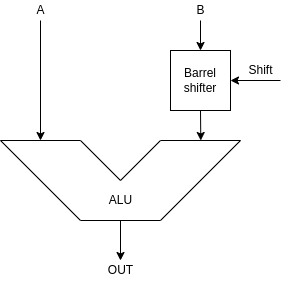
\includegraphics[width=200px]{images/31_ARM/ARM_ALU.png}
\end{figure}
possamo attivare il barrel shifter modificando il terzo parametro:
\begin{verbatim}
    ADD r0, r1, r2 LSL 2
\end{verbatim}
indica che prima di eseguire la somma si deve shiftare a sinistra r2 di 2 posizioni.
Per shiftare e basta posso quindi usare la ADD o la SUB con operandi nulli.

\subsubsection{Operando 2}
L' operando 2 può quindi essere:
\begin{itemize}
    \item un registro
    \item un registro shiftato di un valore fisso
    \item un registro shiftato di un valore contenuto in un registro
    \begin{verbatim}
        ADD r0, r1, r2 LSR r3
    \end{verbatim}
    \item un indirizzamento indiretto
    \begin{verbatim}
        ADD r0, r1, [r2]
    \end{verbatim}
    \item un dato immediato
    \begin{verbatim}
        ADD r0, r1, #9
    \end{verbatim}
\end{itemize}

\subsubsection{Istruzioni condizionali}
Le istruzioni possono aggiornare i flag oppure possono guardarli prima di eseguire le operazioni:
\begin{verbatim}
    ADDEQ r0, r1, r2
        // esegue solo se Z flag è 1
\end{verbatim}

\subsubsection{Indirizzamenti}
Di fatto avendo istruzioni a 32 bit non possiamo avere un indirizzamento immediato o diretto vero e proprio perché non abbiamo posto per indirizzi a 32 bit.
Abbiamo solo 12 bit, quindi gli indirizzi sono codificati utilizzando:
\begin{itemize}
    \item \verb{r{: 4 bit
    \item \verb{b{: 8 bit
\end{itemize}
ed ottenendo l' indirizzo computando \verb{b ROR 2r{.
Posso pertanto creare tutti gli indirizzi ad 8 bit che voglio e poi ruotarli quanto mi pare a destra.

Si noti che questa codifica non spetta al programmatore ma la fa direttamente il compilatore/assemblatore se si può, altrimenti segnala un errore e si deve trovare un' altra soluzione come:
\begin{itemize}
    \item aggiungere altre istruzioni per inserire l' indirizzo in un registro ed utilizzare lui per indirizzamento
    \item utilizzare indirizzamento con offset dal PC:
    \begin{verbatim}
        LDR r0, [NUMERO]
        
        NUMERO:
            .WORD 511
    \end{verbatim}
    possiamo infatti usare 12 bit per indicare un displacement da sommare al registro PC
\end{itemize}

\subsubsection{Calling convention}
Il manuale del processore consiglia anche un determinato passaggio di parametri: si usano i registri r0, r1, r2, r3 in ordine, se ci dovessero essere più parametri si dovrebbero passare tramite lo stack.
Questi registri per le subroutine sono registri scratch quindi sta al chiamante salvarne il contenuto se si dovesse riutilizzarlo dopo la chiamata a funzione.

\subsubsection{Procedura di aggancio}
ARM è una delle poche architetture che alla chiamata a funzione non salva l' indirizzo di ritorno sullo stack ma lo sposta in un registro, in LR.
\begin{verbatim}
    BL r1
        ; branch with link
        ; salta e salva l' indirizzo corrente
        ; lr <- pc
        ; pc <- r1
\end{verbatim}
quindi se la subroutine è una foglia (cioè non chiama altra suprocedure) non salva lr sullo stack, altrimenti deve farlo per poter tornare indietro.
Al posto di una istruzione ret abbiamo:
\begin{verbatim}
    BX r1
        ; pc <- lr
        ; r1 <- pc
\end{verbatim}

\subsection{THUMB}
Questo assembly che abbiamo appena visto tuttavia non è più utilizzato!
Dato che tutte le istruzioni sono a 32 bit abbiamo una code density troppo bassa e programmi troppo grandi, si spreca un sacco di spazio.
Con istruzioni ad 8 bit abbiamo che tante istruzioni non ci stanno quindi devono essere spezzate in più componenti, a 16 bit invece abbiamo un ottimo numero di istruzioni possibili ed una ottima code density.

I processori ARM pertanto forniscono un secondo instruction set detto Thumb, ciò è fatto ponendo un decoder tra il prelievo delle istruzioni e la logica di decodifica ed esecuzione, praticamente Thumb non fa altro che creare degli alias a 16 bit delle istruzioni che ARM già fornisce:
\begin{figure}[H]
    \centering
    
\includegraphics[width=200px]{images/31_ARM/thumb_decoder.png}
\end{figure}
Tuttavia in questa traduzione alcune istruzioni si perdono quindi possiamo dire che Thumb è un subset di ARM.

NB: adesso si usa Thumb-2 che è una versione migliorata che risolve alcuni problemi che aveva Thumb.

NB: alcune istruzioni Thumb sono anche a 32 bit, soprattutto quelle che gestiscono i dati immediati.

\subsubsection{Attivare modalità Thumb}
Per programmarlo si usa la stessa sintassi dell' ARM normale ma l' assemblatore è istruito per tradurre con le codifiche Thumb.

Per attivare la modalità Thumb si usa un flag $T$ nel registro di stato ma non posso attivarlo direttamente tramite qualche istruzioni perché altrimenti creerei problemi alla coda di prefetch che ha già tradotto le prossime istruzioni usando una codifica mentre avrebbe dovuto usare l' altra.
Questo cambio di instruction set viene quindi eseguito durante un salto: in modalità ARM e Thumb le istruzioni sono tutte allineate a multipli di 4 o a multipli di 2 quindi tutti gli indirizzi sono numeri pari, durante il salto si usa il bit meno significativo per specificare l' instruction set di arrivo: supponiamo di dover saltare all' indirizzo 12 se vogliamo che quella subprocedure sia decodificata come thumb inseriamo come indirizzo 13 mentre se voglio che sia decodificato come ARM inseriamo 12.

I Cortex-M4 sono stati i primi processori ARM ad aver eliminato definitivamente la logica e l' instruction set ARM rimanendo solo con Thumb, quindi tutti gli indirizzi di salto e di ritorno saranno dispari (ma questo viene fatto in automatico dall' assemblatore).

\subsection{Gestione degli interrupt}
Il gestore salva direttamente i registri r1-r4 quando si ha una interruzione da gestire.
Possiamo usare una normale funzione in C in quanto di norma il compilatore salva i registri non scratch mentre il gestore salva i rimanenti.

Per agganciare i gestori al processore si deve popolare la tabella dei vettori, è una tabella che si trova a partire dall' indirizzo 0 e deve contenere gli indirizzi delle procedure che si vogliono usare come gestori.

I primi 16 gestori sono riservati al core per gestire le eccezioni, mentre da 16 in poi sono interruzioni lasciate per le periferiche che si vogliono installare nel chip. 

\subsubsection{Eccezioni}
L' indirizzo 0 al reset deve contenere l' SP iniziale, l' indirizzo 1 contiene l' indirizzo del vettore di reset, successivamente ci sono altre interruzioni come:
\begin{itemize}
    \item divisione per zero
    \item accesso non allineato
    \item accesso a zona di memoria non mappata
    \item svc: provoca un fault nel processore e si utilizza per chiamare il sistema operativo
    \item hard fault
\end{itemize}

\subsubsection{Hard fault}
E' una eccezione che si verifica quando c'è una eccezione all' interno di un gestore, abbiamo cioè un fault dentro un fault.
Se a sua volta c'è una eccezione interna all' hard fault abbiamo un triplo fault!
Se succede un triplo fault il processore si blocca e mette a livello alto un certo pin, di solito attaccato ad un led per notifica.

L' occasione standard di un hard fault si ha quando ci sono dei gestori non inizializzati: arriva una eccezione che non ho previsto, trovo zero come vettore, salto all' hard fault, magari trovo zero come vettore perché non l'ho implementato ed ho triplo fault.

Di solito per motivi di debug si usa un hard fault con il codice:
\begin{verbatim}
    hard_fault {
        while(1);
    }
\end{verbatim}
e tramite dispositivi di debug si analizza il perché delle problematiche.